

%\vspace{-15pt}
\begin{IEEEbiography}[{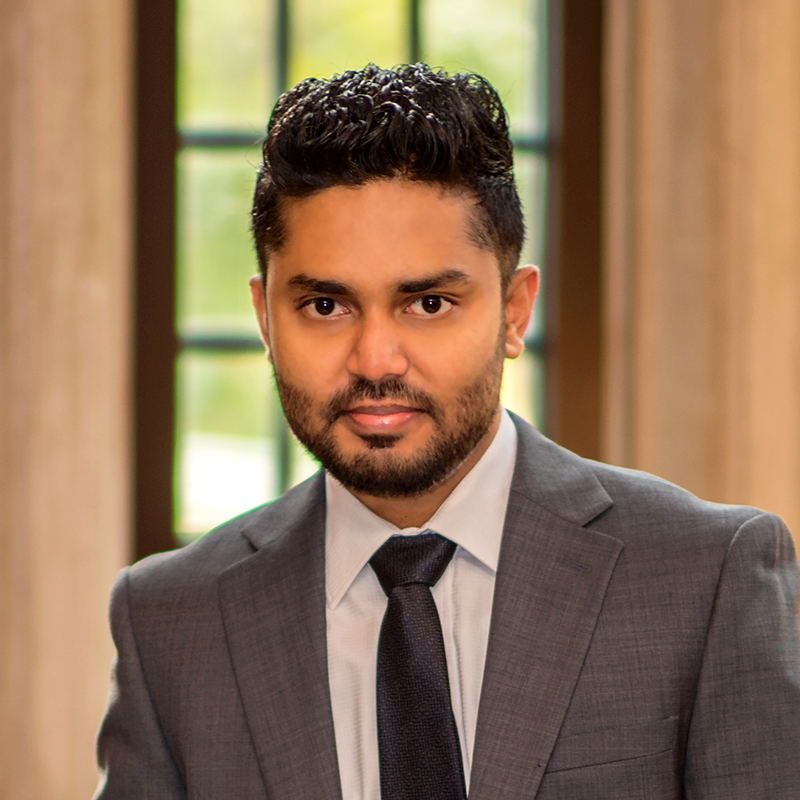
\includegraphics[width=1in,height=1.25in,clip,keepaspectratio]{bios/Kadupitiya_JCS.jpg}}]
{JCS Kadupitiya} is a Ph.D. candidate in the Department of Intelligent Systems Engineering at Indiana University Bloomington. He received a Master's in Computer Engineering from Indiana University Bloomington in 2019.  His research interests lie primarily in scientific machine learning and distributed computing. He completed his Bachelor’s degree in Electrical and Information Engineering from the University of Ruhuna, Sri Lanka, in 2015. He also received a Master's in Computer Science and Engineering at the University of Moratuwa, Sri Lanka, in 2017.
\end{IEEEbiography}


\begin{IEEEbiography}[{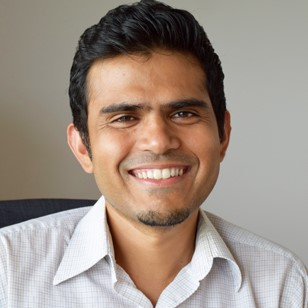
\includegraphics[width=1in,height=1.25in,clip,keepaspectratio]{bios/jadhao-vikram-2016-08.jpg}}]
 {Vikram Jadhao} is an assistant professor of Intelligent Systems Engineering at Indiana University in Bloomington. Prior to joining Indiana University, he held postdoctoral fellowships in the Department of Physics and Astronomy at Johns Hopkins University as well as the Department of Materials Science and Engineering at Northwestern University. He received his Ph.D. and M.S. in Physics from the University of Illinois at Urbana-Champaign, and his B.S. in Physics from the Indian Institute of Technology at Kharagpur. His research interests are broadly in computational modeling and simulation of soft materials at the nanoscale. 
\end{IEEEbiography}


%\vspace{-15pt}

\begin{IEEEbiography}[{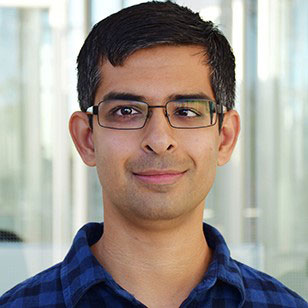
\includegraphics[width=1in,height=1.25in,clip,keepaspectratio]{bios/prateeks.jpg}}]{Prateek Sharma}
  is an an assistant professor of Intelligent Systems Engineering at Indiana University in Bloomington. He has a PhD in Computer Science from 
the University of Massachusetts Amherst. His current research
  focuses on Cloud Computing, Operating Systems, and
  Virtualization. Sharma received his masters degree in Computer Science from
  Indian Institute of Technology, Bombay. Contact him at
  prateeks@iu.edu.
\end{IEEEbiography}

%\vspace{-10pt}



%%% Local Variables:
%%% mode: latex
%%% TeX-master: "paper"
%%% End:
